\chapter{\label{III-B}Le \ldd de l’\ac{ina} : le référentiel au centre du modèle}
\titreEntete{Le référentiel au centre du modèle}

%intro
\lettrine{L}'impact du \ac{lod} sur la structure des données et l'éclatement des référentiels a été l'un des aspects de la refonte des systèmes d'information en institutions ou en entreprises, sous la forme de \ac{led}. Ces \ac{led} sont des modèles de données à la structure similaire au \ac{lod}, ce qui les rend très efficaces et utiles dans l'utilisation des données qui en découle.\\

Le \ldd de l'\ac{ina} est l'un de ces \ac{led}: il a vocation à regrouper l'ensemble des métadonnées de l'Institut, en provenance, sous diverses formes, de plusieurs départements.  L'opération de traitement, nécessaire pour la création de ce \textit{Lac}, permet de enrichir ces métadonnées par de multiples liens avec le \ac{lod} ou des référentiels internes: le lien devient une notion prioritaire et essentielle entre des données d'un même document qui sont éclatées en plusieurs instances ou concepts.

\section{\label{III-B-1}Application des principes du Web de données aux systèmes documentaires: le Linked Enterprise Data}
\titreEntete{Le Linked Enterprise Data}

%intro
L'apport du Web de données à la structure des données et à la place des référentiels est important. Lier un système documentaire au Web de données est possible; repenser ce système documentaire selon les principes du Web de données pour s'adapter aux nouveaux besoins et aux nouveaux usages est une pratique de plus en plus courante dans les institutions patrimoniales. L'\ac{ina} a ainsi entrepris une réflexion sur cette transformation dès 2012, et sa mise en œuvre en 2015. Face à l'accumulation de bases de données, un modèle de données inspiré du Web de données doit pouvoir recentraliser les métadonnées et assurer l'interopérabilité de l'ensemble du système documentaire.\\

L'interopérabilité du système --- uniquement celui de l'\ac{ina}, il n'est pas nécessaire ni envisageable de le rendre interopérable avec les autres institutions et le Web de données --- est seulement possible par le repositionnement du référentiel en son sein.

\subsection{\label{III-B-1-a}Permettre l'interopérabilité au sein des institutions}
\titreEntete{Permettre l'interopérabilité au sein des institutions}

L'interopérabilité du système documentaire est le principal enjeu du \ldd. Nous l'avons évoque au \reference{I-B}, l'\ac{ina} possède plusieurs bases de données distinctes, propres à chaque métier et à chaque besoin. Les référentiels ne sont communs qu'entre les métiers aux mêmes besoins: la \ac{dj} et la \ac{ddcol} ne partagent pas le même référentiel de personnes physiques et morales; il existe par conséquent deux de ces référentiels au sein d'une même institution.\\

La création d'un LED permet de centraliser ces référentiels et de les partager entre les différents corps de métier, qu'ils soient juridiques, patrimoniaux ou commerciaux. Elle permet également de casser le monolithisme\footnote{Terme employé par \nP{Emmanuelle}{Bermès}, \nP{Gautier}{Poupeau} et \nP{Antoine}{Isaac} dans \cite{bermes_cas_2013}} du système documentaire, pensé comme un tout répondant à un besoin à un instant précis. Seulement, l'évolution des usages, l'évolution des usages, et l'évolution des documents à décrire, entraînent une modification de la description qui est réalisée, et par conséquent une sédimentation de rajouts aux bases de données sources. En effet, étant conçues pour un unique besoin, ces bases supportent mal les modifications de modèle de données, ce qui créé de nouveaux attributs dans les tables, ou bien de nouvelles tables dans les bases de données.\\

Les difficultés posées par ces multiples bases de données concernent également l'utilisation qui est faite des métadonnées. De même que des portails sont des moyens d'assurer une interopérabilité --- par plus petit dénominateur commun --- entre deux jeux de données du Web de données, l'application Hyperbase de l'\ac{ina} permet de consulter les données des bases \ac{da} et \ac{dl}\footnote{Voir \reference{annexe_bdd_ina} (\reference{bdd_ddcol_ina}).}. Mais cette application comble seulement partiellement des différences de modélisation des données dans chacune des bases de données. La création de cette application répondait au besoin de pouvoir consulter sur une même page des données provenant de diverses bases. De nombreuses autres applications ont été créées pour répondre rapidement, chacune, à un besoin: Totem pour le \ac{da} ou MediaIndex pour le \ac{dl} sont deux exemples de ces applications aux usages similaires propres à chaque métier.\\

L'utilisation d'un LED permet de retourner l'utilisation qui est faite d'un système documentaire: plutôt que de partir des besoins et des usages qui seront faits des données, la réflexion se porte d'abord sur les données afin de bâtir un modèle de données qui puisse s'adapter à l'évolution des besoins, sans avoir besoin de les prévoir.  Le LED rend leur cohérence aux données et aux informations, permet une meilleure gestion de ces données et informations, et une amélioration des services rendus à l'utilisateur final.

\subsection{\label{III-B-1-b}Repenser le système documentaire}
\titreEntete{Repenser le système documentaire}

L'objectif du LED est l'interopérabilité, la connexion entre les jeux de données de l'institution, ou de l'entreprise, qui ont des structures différentes mais partagent des points communs comme les référentiels. Pour cela, les processus ETL (Extract-Transform-Load) sont essentiels. De multiples bases de données, l'objectif est d'en obtenir une seule en conservant la totalité des données migrées. Au cours de ce traitement pour restructurer chaque donnée, il est possible d'apporter un enrichissement au travers d'alignements avec d'autres jeux de données ou référentiels. Ces alignements, nous l'avons montré, peuvent être de deux types:
\begin{itemize}
	\item internes, entre deux jeux de données de l'institution\footnote{Voir \reference{I-C-3}.} pour assurer l'interopérabilité du système
	\item externes, entre un jeu de données de l'institution et un jeu de données d'une autre institution grâce au Web de données\footnote{Voir \reference{II-C} et \reference{III-A-3}.}
\end{itemize}
\medskip

En repensant le système documentaire depuis les données au lieu des besoins et des usages qui en seront faits, de multiples usages peuvent naître et sont facilités dans leur développement par la centralisation des données: à l'\ac{ina}, le \ldd permet d'alimenter plusieurs applications et sites Web, comme \href{https://www.ina.fr//}{ina.fr}, \href{https://madelen.ina.fr/}{madelelen.ina.fr} ou \href{https://www.inamediapro.com}{inamediapro.fr}. De même que dans le Web de données, chaque document, chaque instance de l'\ac{ina} et du LED se voit attribuer un identifiant unique, facilitant ainsi l'établissement de liens entre les instances, ou avec les référentiels. Ces identifiants permettent une interopérabilité par les liens, similaire au Web de données: ainsi, l'interopérabilité du LED ne passe pas, comme cela pouvait être le cas en bibliothèque avec le format \ac{marc}, par une interopérabilité par un format unique.

\subsection{\label{III-B-1-c}Le positionnement du référentiel}
\titreEntete{Le positionnement du référentiel}

La création des liens entre les instances du LED nécessite, lors du processus d'ETL, d'utiliser des référentiels ou de trouver les points de contacts entre les jeux de données. Ces référentiels deviennent des pivots dans le système documentaire: le \ac{da} et le \ac{dl} partagent des structures de données différentes; pourtant, des liens entre ces deux jeux de données peuvent être établis grâce aux référentiels --- celui des personnes physiques et morales, celui des types de matériels, le thésaurus des noms communs, \dots~ Utiliser des référentiels pour établir du lien ne nécessite pas d'alignement entre les données puisque les tables des bases de données sont déjà liées aux référentiels. En revanche, l'utilisation des points de contact nécessite la réalisation d'alignements, de manière à recoller deux mêmes concepts ou instances de deux jeux de données ou de deux référentiels.\\

La création d'un référentiel commun dans le LED apparaît par conséquent nécessaire et indispensable. Cependant, ce référentiel peut ne pas être créé spécifiquement pour le LED, mais être une réutilisation d'un référentiel existant dont on aurait décidé de manière commune que sa valeur est supérieure à un autre: dans le cas des référentiels des personnes physiques de l'\ac{ina}, un choix doit être fait pour décider lequel des référentiels de personnes de la \ac{ddcol} ou de la \ac{dj} imposera ses normes de graphie. De même, des choix doivent être effectués quant aux référentiels externes utilisés: Wikidata est une base de connaissances globale comprenant plusieurs dizaines de millions d'entités, mais cette base n'est pas assez complète pour pouvoir être utilisée à l'\ac{ina} comme référentiel commun sur lequel l'ensemble des données repose. En effet, nous l'avons montré lors de l'alignement des personnes physiques avec Wikidata, de nombreuses personnes, peu ou pas connues, ne font pas l'objet d'une entité Wikidata: l'\ac{ina} ne peut alors qu'enrichir ses données avec l'identifiant de Wikidata, ou avec d'autres identifiants extraits de Wikidata grâce au hub de liens et d'identifiants que représente cette base de connaissances. Le repositionnement des référentiels au centre du système documentaire permet ainsi d'éviter les redondances de données entre les bases.\\

Cependant, nous le verrons ensuite (\reference{III-B-2}), la présence d'un référentiel défini comme référentiel n'est pas indispensable. En effet, comme dans le Web de données, le référentiel s'est progressivement disloqué en données avec les modèles en graphe, faisant alors de chaque référentiel un jeu de données comme les autres. Plus encore, un jeu de données qui n'est pas défini comme référentiel peut à son tour devenir référentiel s'il est utilisé et lié avec une autre donnée.

%conclu
\bigskip
\bigskip

L'impact du Linked Enterprise Data est multiple, mais contribue notamment à posséder une base de données cohérente et structurée, laquelle ne dépend pas des utilisations qui en sont faites. Ainsi, une application utilise la base de données et sa structure, sans avoir d'incidence sur le stockage et la gestion des données. Le LED permet alors une grande évolutivité du système dans ses modifications.
\section{\label{III-B-2}Le \ldd de l'\ac{ina}: un repositionnement du référentiel au centre du modèle de données}
\titreEntete{Le \ldd de l'INA}

%intro
La fusion du \ac{dl} et du \ac{da} dans la \ac{ddcol} en 2012 n'ont pas permis de centraliser les deux silos de données existants. Ainsi, en 2015, le projet du \ldd~ est lancé afin de centraliser les données et les métadonnées de tout l'Institut, afin de les mettre en cohérence, de supprimer les redondances et les barrières techniques ou structurelles de ces données, de répondre enfin aux nouveaux enjeux de la fin des années 2010.\\

Un nouveau modèle de données, construit sur le contenu intellectuel et non les usages, et accompagné d'une nouvelle infrastructure centralisée pour l'accueil des données et des métadonnées, voit le jour. Le référentiel, déconstruit, devient une donnée identique aux données résultant de la décomposition de la notice documentaire. Au-delà de ce modèle de données, c'est l'ensemble du système d'information qui subit cette refonte, avec un stockage des données, leur traitement et des accès repensés.

\subsection{\label{III-B-2-a}Le \ldd, un modèle basé sur des classes d'entités}
\titreEntete{Un modèle basé sur des classes d'entités}

Le Web de données avait permis la déconstruction des informations en données, l'effacement du référentiel au profit de données déstructurées mais liées. La réflexion sur le nouveau modèle de données de l'\aca{ina} a conduit au même phénomène: les données bibliographiques --- de description des documents audiovisuels --- se retrouvent au même niveau que les données d'autorités issues des référentiels. Les données d'autorités ne se trouvent plus à la marge du système documentaire, mais bien intégrées dedans, au centre, puisqu'elles deviennent indispensables dans la description des documents.\\

Le modèle de données du \ldd~ propose une structure globale, et adaptable à chaque besoins non pensés lors de la modélisation, pour accueillir les données. Pour cela, le modèle du \ldd~ est basé sur les relations entre cinq principales classes d'entités (\footnote{Voir \reference{annexe_nvx_modeles} (\reference{modele_ldd}).}). En cela, ce modèle peut ressembler aux \ac{frbr}\footnote{Présentés précédémment dans la \reference{II-A-1}.} avec ses quatre grandes classes item, manifestation, expression et œuvre; le modèle du \ac{cidoccrm} ou d'autres modèles à entités peuvent également être comparés. Le \ldd~ n'adopte aucun des modèles de données existant dans le domaine bibliothéconomique ou patrimonial en raison de la spécificité des fonds conservés et des données documentaires produites, ainsi que de la singularité de l'historique de la \ac{ddcol} qui conserve à la fois des données orientées événement ou archivistiques.


\noindent L'\textbf{instance} est la première des cinq entités principales du \ldd. Elle correspond à l'entité intellectuelle du contenu --- un programme, qu'il soit par exemple une émission, ou bien un reportage; une photographie; une documentation d'accompagnement, un épisode de série ou une fiction, \dots): sans l'être exactement, l'instance peut être rapprochée de l'œuvre des \ac{frbr}.


\noindent L'\textbf{événement} permet la description d'un événement attaché à une instance: cet événement peut être lié à la création du contenu (la captation, l'enregistrement, la prise de vue pour une photographie, \dots), à l'exploitation qui en a été faite (diffusion télévisuelle, projection des \textit{Actualités françaises} au cinéma, mise en ligne sur l'une des plateformes de l'\ac{ina}, \dots), ou bien à l'archivage et à l'usage de ce contenu (numérisation, restauration, description des droits et des informations juridiques pesant sur le contenu, \dots).

\noindent L'\textbf{item} correspond au matériel --- physique ou numérique --- sur lequel se trouvent les contenus (bandes LTO du dépôt légal, photographie, \dots).

\noindent Les \textbf{textes} permettent une description du contenu par le langage naturel: il peut s'agir de titres extraits de génériques ou saisis par le technicien de gestion des collections multimédia lors du catalogage; les identifiants sont également des textes; \dots ~ Ces textes ne sont pas soumis aux référentiels et ne les constitue pas.

\noindent Le \textbf{concept} est le pivot du modèle de données puisqu'il représente les référentiels. Il permet la description de toutes les instances.\\

L'identification de chacune de ces entités est nécessaire puisque le modèle de données du \ldd~ est conçu à partir de relations entre ces entités: le Web de données dispose d'URIs HTTP, ce modèle de données d'une entreprise utilise des identifiants non significatifs (il s'agit d'une suite de douze chiffres et lettres) pour créer du lien au sein de son système documentaire (\reference{schema_ldd_1}).

\begin{figure}[!h]
	\centering
	\begin{pspicture}(0,0)(15.2,6)
		\psframe[fillstyle=solid,fillcolor=lightgray](12,0)(15,1)
		\psframe[fillstyle=solid,fillcolor=lightgray](12,3)(15,4)
		\psframe[fillstyle=solid,fillcolor=lightgray](6,3)(9,4)
		\psframe[fillstyle=solid,fillcolor=lightgray](0,1.5)(3,2.5)
		\psframe[fillstyle=solid,fillcolor=lightgray](0,4.5)(3,5.5)
		
		\psline(9,3.5)(12,3.5)
		\psline(13.5,3)(13.5,1)
		\psline(3,2)(4.5,2)
		\psline(4.5,2)(4.5,3.4)
		\psline(4.5,3.4)(6,3.4)
		\psline(3,5)(4.5,5)
		\psline(4.5,5)(4.5,3.6)
		\psline(4.5,3.6)(6,3.6)
		\psline(1.5,4.5)(1.5,2.5)
		\psline(9,3.2)(10.5,3.2)
		\psline(10.5,3.2)(10.5,0.5)
		\psline(10.5,0.5)(12,0.5)
		
		\uput[0](0.8, 4.9){\textit{Texte}}
		\uput[0](0.55,1.9){\textit{Concept}}
		\uput[0](6.55,3.4){\textit{Instance}}
		\uput[0](12.3,3.4){\textit{Événement}}
		\uput[0](12.8,0.4){\textit{Item}}
	\end{pspicture}
	\caption{Modélisation des cinq entités du \ldd}
	\label{schema_ldd_1}
\end{figure}

\subsection{\label{III-B-2-b}La place des concepts}
\titreEntete{La place des concepts}

Le modèle de données établi dans le \ldd permet de ne créer qu'un seul \og référentiel\fg{} grâce aux concepts. Ces derniers permettent la description de l'ensemble des instances: dans ce modèle, un grand nombre de données sont comprises comme des concepts. C'est pourquoi ils regroupent une grande variété de noms communs et de noms propres dont:
\begin{itemize}
	\item les personnes physiques et morales, tirées du référentiel des personnes physiques et morales de la \ac{ddcol}
	\item les noms communs issus du thésaurus des noms communs de cette même \ac{ddcol}: ils offrent les autorités matière nécessaires à la description (l'instance concerne-t-elle le sport? la télévision? la cuisine? \dots)
	\item  le genre de l'instance (émission, reportage, film, épisode de série, fiction, \dots)
	\item la provenance de l'instance, ce qui concerne notamment les codes des chaînes de télévision et des stations de radio employés dans les bases sources et repris dans le \ldd, mais concerne également la base source de provenance des données du \ldd. En effet, la migration de données depuis une base vers une source nécessite de conserver la trace de son parcours afin de repérer d'éventuelles erreurs de mapping: ainsi, les codes des bases sources sont ainsi des concepts.
	\item etc.\footnote{Plusieurs millions de données sont devenus des concepts dans le nouveau système documentaire de l'\ac{ina}.}
\end{itemize}
\medskip

Les entités du \ldd sont similaires aux entités de Wikidata par la nécessité de la création de liens entre elles afin qu'elles puissent exister dans le modèle de données. Afin de relier ces cinq entités et de mettre en cohérence les données, des relations typées sont créés entre les entités, notamment entre les concepts, de manière à identifier le rôle, le type, ou la fonction du concept par rapport à l'instance ou au texte. Ainsi, des tables permettent, comme pour les annotations ou les crédits, de lier des concepts aux instances afin d'apporter du sens. De plus, il est possible avec ce modèle de données d'établir une relation entre deux concepts, afin d'exprimer par exemple la provenance d'un concept d'une personne (\reference{schema_concept_1}). 
\begin{figure}
    \centering
    \begin{pspicture}(0,0)(15,5)
        \psframe[fillstyle=solid,fillcolor=lightgray](0,0)(3,1)
        \psframe[fillstyle=solid,fillcolor=lightgray](6,2.5)(9,3.5)
        \psframe[fillstyle=solid,fillcolor=lightgray](12,0)(15,1)
        
        \psline(9,3.1)(10,3.1)
        \psline(10,3.1)(10,4.6)
        \psline(10,4.6)(8,4.6)
        \psline{->}(8,4.6)(8,3.5)
        \uput[0](6.7, 3){\textit{Concept}}
        
        \uput[0](0.7,0.5){\textit{Instance}}
        
        \uput[0](12.9,0.5){\textit{Texte}}
        
        \uput[0](5.3,1){Crédit}
        \psline(3,1)(5.2,1)
        \psline(6,1.4)(6,2.5)
        \uput[0](3.3,1.7){Annotation}
        \psline(3,1)(4,1.4)
        \psline(5,2)(6,2.5)
        \uput[0](2.2,3){Relation}
        \psline(3,1)(3,2.6)
        \psline(3.6,3)(6,3)
    
        \uput[0](10,1.8){Label}
        \psline(12,1)(11.1,1.5)
        \psline(10,2)(9,2.5)
    \end{pspicture}
    \caption{Modélisation globale des relations entretenues par les concepts}
    \label{schema_concept_1}
\end{figure}

L'établissement de relations entre les entités n'est possible qu'avec les identifiants attribués à chacune des entités. Un concept n'est par conséquent pas défini dans un seul endroit, à une seule table: un graphe de relations se met en place tout autour de lui afin de le définir le plus précisément et de lui apporter du contexte et du sens. Ces relations internes sont essentielles au fonctionnement du système documentaire et de la cohérence(\reference{schema_concept_2}).
\begin{figure}
    \centering
    \begin{pspicture}(0,0)(17,9.6)
        \psframe[fillstyle=solid,fillcolor=green!60](7,5)(10,6)
        \uput[0](7.8,5.5){abcd1}
        \psframe[fillstyle=solid,fillcolor=green!60](10.5,7.5)(13.5,8.5)
        \uput[0](11.4,8){h5ds6}
        \psline(8.5,6)(12,7.5)
        \uput[0](9.5,6.7){\textit{provenance}}
        \psframe[fillstyle=solid,fillcolor=green!60](0,8.5)(3,9.5)
        \uput[0](0.9,9){sg62fg}
        \psframe[fillstyle=solid,fillcolor=green!60](14,2.5)(17,3.5)
        \uput[0](14.9,3){aefd2}
        
        \psframe[fillstyle=solid,fillcolor=yellow!60](14,6.25)(17,7.25)
        \uput[0](15.1,6.75){PP}
        \psline(13.5,8)(15.5,7.25)
        \uput[0](14,7.7){\textit{label}}
        \psframe[fillstyle=solid,fillcolor=yellow!60](13,4.6)(16,5.6)
        \uput[0](13.1,5.1){Farmer, Mylène}
        \psline(10,5.4)(13,5.1)
        \psline(14.5,4.6)(15.5,3.5)
        \uput[0](10.8,5.3){\textit{label}}
        \uput[0](14,4){\textit{provenance}}
        \psframe[fillstyle=solid,fillcolor=yellow!60](9,2.7)(12,3.7)
        \uput[0](9.6,3.2){10132989}
        \psline(12,3.2)(14,3)
        \psline(8.5,5)(10.5,3.7)
        \uput[0](8.8,4.2){\textit{identifiant}}
        \uput[0](12,2.9){\textit{provenance}}
        \psframe[fillstyle=solid,fillcolor=yellow!60](14,0)(17,1)
        \uput[0](15,0.5){DA}
        \psline(15.5,2.5)(15.5,1)
        \uput[0](15,1.65){\textit{label}}
        \psframe[fillstyle=solid,fillcolor=yellow!60](5,7.5)(8,8.5)
        \uput[0](4.9,8){\footnotesize{GAUTIER MYLENE}}
        \psline(8.5,6)(6.5,7.5)
        \psline(5,8)(3,9)
        \uput[0](7,6.8){\textit{label}}
        \uput[0](3,8.4){\textit{provenance}}
        \psframe[fillstyle=solid,fillcolor=yellow!60](0,6.25)(3,7.25)
        \uput[0](1.1,6.7){DJ}
        \psline(1.5,8.5)(1.5,7.25)
        \uput[0](1,7.7){\textit{label}}
        
        \psframe[fillstyle=solid,fillcolor=blue!30](1,3)(4,4)
        \uput[0](1.9,3.5){ss6fdb}
        \psline(5.5,2)(8.5,5)
        \uput[0](5.9,3){\textit{crédit}}
        \psframe[fillstyle=solid,fillcolor=blue!30](4,1)(7,2)
        \uput[0](4.9,1.5){18f6yu}
        \psline(4,3.5)(7,5.5)
        \uput[0](4.9,4.6){\textit{crédit}}
    \end{pspicture}
    \caption[Modélisation du concept \nP{Mylène}{Farmer} dans le \ldd]{Modélisation du concept \nP{Mylène}{Farmer} dans le \ldd [Données partielles d'exemple. Vert: concept. Jaune: texte. Bleu: instance.]}
    \label{schema_concept_2}
\end{figure}

Le modèle de données du \ldd lui permet également d'obtenir une ouverture à l'extérieur, vers le Web de données, afin d'obtenir des informations et des données supplémentaires. Ainsi, la simple conservation de quelques identifiants comme ceux de Wikidata ou de la BnF, et des identifiants internationaux comme l'\ac{isan} suffisent à créer des ponts avec le Web de données(\reference{schema_concept_3}).
\begin{figure}
    \centering
    \begin{pspicture}(7,0)(24.2,17)
        \psframe[fillstyle=solid,fillcolor=green!60](7,7.5)(10,8.5)
        \uput[0](7.8,8){abcd1}
        \psframe[fillstyle=solid,fillcolor=green!60](14,2.5)(17,3.5)
        \uput[0](14.9,3){aefd2}
        \psframe[fillstyle=solid,fillcolor=yellow!60](14,5)(17,6)
        \uput[0](14.1,5.5){Farmer, Mylène}
        \psline(10,8)(14.4,6)
        \psline(15.5,5)(15.5,3.5)
        \uput[0](11.8,6.7){\textit{label}}
        \uput[0](14.4,4.3){\textit{provenance}}
        \psframe[fillstyle=solid,fillcolor=yellow!60](10,3.75)(13,4.75)
        \uput[0](10.6,4.25){10132989}
        \psline(11.5,3.75)(14,3)
        \uput[0](11.6,3.3){\textit{provenance}}
        \psline(11.5,4.75)(8.5,7.5)
        \uput[0](8.6,6.2){\textit{identifiant métier}}
        \psframe[fillstyle=solid,fillcolor=yellow!60](14,0)(17,1)
        \uput[0](15,0.5){DA}
        \psline(15.5,2.5)(15.5,1)
        \uput[0](15,1.65){\textit{label}}
        \psframe[fillstyle=solid,fillcolor=blue!30](7,1)(10,2)
        \uput[0](7.9,1.5){ss6fdb}
        \psline(8.5,2)(8.5,7.5)
        \uput[0](7.9,4.2){\textit{crédit}}
        \psframe[fillstyle=solid,fillcolor=yellow!60](7,10)(10,11)
        \uput[0](7.65,10.5){Q185002}
        \psline(8.5,8.5)(8.5,10)
        \uput[0](6.7,9.2){\textit{identifiant Wikidata}}
        \psframe[fillstyle=solid,fillcolor=yellow!60](14,7.5)(17,8.5)
        \uput[0](14.2,8){cb13893800r}
        \psline(10,8)(14,8)
        \uput[0](11,8.1){\textit{identifiant BnF}}
        \pscurve[linewidth=0.06](7,11.5)(11,11.5)(17.5,9)(17.5,0)
        \uput[0](11.2,1.5){\huge{\textbf{LED}}}
        
        \uput[0](20.2,1.5){\huge{\textbf{LOD}}}
        \psframe(14,13)(17,14)
        \uput[0](14.7,13.5){Q185002}
        \psline[linestyle=dashed](10,11)(14,13)
        \psframe(10,15.5)(13,16.5)
        \uput[0](10.5,16){1961-09-12}
        \psline(14,14)(11.5,15.5)
        \uput[0](12,14.9){\textit{P569}}
        \psframe(17.5,15.5)(20.5,16.5)
        \uput[0](18.3,16){Q2360927}
        \psline(17,14)(19,15.5)
        \uput[0](17.8,14.8){\textit{P19}}
        \psframe(21,13)(24,14)
        \uput[0](21.5,13.5){Pierrefonds}
        \psline(20,15.5)(22.5,14)
        \uput[0](20.5,14.6){\textit{skos:label}}
        \psframe(17.5,11)(20.5,12)
        \uput[0](18.2,11.5){85395788}
        \psline(17,13)(19,12)
        \uput[0](17.4,12.5){\textit{P214}}
        \uput[0](10.5,13.5){\Large{\textbf{Wikidata}}}
        \psframe(21,9)(24,10)
        \uput[0](21.7,9.5){85395788}
        \psline[linestyle=dashed](19,11)(22.5,10)
        \uput[0](19,9.5){\Large{\textbf{VIAF}}}
        
        
        \psframe(19,7)(22,8)
        \uput[0](19.4,7.5){cb13893800r}
        \psline[linestyle=dashed](17,8)(19,7.5)
        \psline[linestyle=dashed](22.5,9)(20.5,8)
        \uput[0](19.4,6.2){\Large{\textbf{BnF}}}
        
        \psframe(21,4)(24,5)
        \uput[0](21.4,4.5){073924784}
        \psline[linestyle=dashed](23,9)(23,5)
        \uput[0](20.2,3.2){\Large{\textbf{Sudoc}}}
        
    \end{pspicture}
    \caption[Modélisation du concept \nP{Mylène}{Farmer} dans le \ldd et le LOD]{Modélisation du concept \nP{Mylène}{Farmer} dans le \ldd et le LOD [Données partielles d'exemple. Vert: concept. Jaune: texte. Bleu: instance.]}
    \label{schema_concept_3}
\end{figure}

\subsection{\label{III-B-2-c}Le \ldd comme un LED: une infrastructure unique}
\titreEntete{Une infrastructure unique}

\begin{citationLongue}
	À l’heure où nous cherchons à faire fructifier la donnée, comme actif de l’entreprise, il est essentiel pour réussir justement à faire émerger de nouveaux usages de décloisonner nos silos de données et de libérer la donnée de l’usage pour lequel elle a initialement été créée.\footcite{poupeau_reflexions_2018}
\end{citationLongue}

Le \ldd n'est pas seulement la refonte d'un modèle de données. Afin de disposer des capacités de stockage, de traitement, et d'accès nécessaires, le \ldd est également la création d'une infrastructure centralisée, depuis laquelle les applications futures pourront être créées: en cela, il est un LED, pensé depuis le bas, depuis les donneés, afin de permettre une multiplicité d'applications\footnote{Voir \reference{annexe_lac} (\reference{lac_infra}).}.\\

La couche la plus basse de ce LED est la base de données. Le choix de celle-ci est essentiel afin de lier performance et modèle de données. Ainsi, chaque type de base de données ayant ses propres caractéristiques, ses propres avantages et ses limites, l'\ac{ina} utilise les quatre types de bases de données en y dupliquant le modèle de données. Alors, le modèle de données est respecté et les applications nécessitant de la part des bases de données de grandes performances pourront en utiliser une plutôt qu'une autre:
\begin{itemize}
	\item les bases de données relationnelles offrent une forte structuration de la donnée, et de bonnes performances d'écriture et de lecture --- ce qui avait conduit à leur adoption par le \ac{da}, le \ac{dl} ou la \ac{dj}. Cependant, la création de relations entre les entités nécessite la création de nombreuses tables et l'éparpillement de la donnée dans la base; les calculs nécessaires pour rassembler les données d'une entité deviennent complexes et longs, ce qui rend la base de données relationnelle peut performante pour le \ldd
	\item la base de données document permet quant à elle une montée en charge rapide et importante avec la possibilité de conserver de grandes masses de documents, mais ne permet pas le respect de la structuration des données
	\item le moteur de recherche permet également cette montée en charge, ainsi qu'une recherche plein texte efficace et rapide obtenue par l'indexation des données dans le moteur
	\item enfin, la base de données graphe permet une structuration très fine des données obtenue par les liens établis entre ces données; cependant, de même que les bases de données relationnelles, la performance lors des requêtes est très vite limitée dès que les requêtes se complexifient et ont pour but de restituer l'intégralité des informations concernant un document, un concept, \dots
\end{itemize}
\medskip

Pour tirer les avantages de chacun de ces types de bases de données, le choix a été fait de les utiliser tous les quatre en y dupliquant les données. Ce choix, dans un LED, ne pose pas de difficultés pour la couche supérieure qui est le traitement des données. En effet, les processus ETL --- et notamment le logiciel Talend qui permet de les développer --- sont créés pour effectuer des extractions de plusieurs bases de données différentes afin de retourner des données transformées, structurées et adaptées aux besoins de la couche supérieure, l'accès aux données pour l'utilisateur. La phase d'accès à ces données n'a alors pas directement accès aux bases sources, mais les obtient par la couche d'abstraction qui est la phase de traitement.

%conclu
Par le \ldd, l'\ac{ina} trouve une cohérence dans ses données, les différences existantes entre les diverses bases de données de la \ac{ddcol} et de la \ac{dj} notamment, ainsi qu'au sein même de la \ac{ddcol} avec le \ac{da} et la \ac{dl}, sont effacées au profit d'une individualité de la donnée obtenue par la déconstruction des documents et de l'information. L'effacement de ces différences permet également de normaliser les données autour de mêmes concepts, et ainsi de créer un graphe dans lequel il est possible de circuler entre instances partageant un même concept.\\

Ces avancées ont été obtenues par le renversement de la pensée du système documentaire et de la place du référentiel. En effet, au lieu de penser la structure des données selon les besoins et les usages finaux --- ce qui créé nécessairement autant de structures que de besoins et d'usages ---, la réflexion a été retournée pour penser un modèle de données global et unique au sein de l'institution depuis les données elle-mêmes et le contenu intellectuel, depuis les documents conservés à l'\ac{ina}, eux qui sont l'essence de l'Institut.
\section{\label{III-B-3}Perspectives d'utilisation}
\titreEntete{Perspectives d'utilisation}

%intro
\begin{citationLongue}
	[L]e rôle central du référentiel va se poursuivre au-delà de [la] réflexion sur l’interopérabilité. En effet, ils sont la pierre angulaire des nouveaux bouleversements autour du \textit{machine learning} et du \textit{deep learning}.\footcite{poupeau_reflexions_2018}
\end{citationLongue}

L'interopérabilité des données --- comprises au sens large, avec les métadonnées et les référentiels --- est une avancée majeure dans la conception des modèles de données. En effet, en plus de résoudre les nombreuses difficultés qui résultaient de la multiplicité des bases de données à l'\ac{ina} et de leur conception par les besoins et les usages qui en étaient faits, la centralisation de ces données et leur interopérabilité ouvre des possibilités quant aux nouveaux usages qu'il est possible d'envisager ou de satisfaire.\\

L'intégration de l'\ac{ina} dans le \textit{big data} est l'une de ces possibilités: l'utilisation de l'intelligence artificielle permet à la fois une amélioration des descriptions déjà réalisées au catalogage, et ainsi que la création de nouvelles descriptions. Plus encore que ces actions sur les métadonnées et la création de descriptions de contenus, l'amélioration de la valorisation des documents de l'\ac{ina} est possible avec le \ldd et l'uniformisation du modèle de données.

\subsection{\label{III-B-3-a}Permettre l’intégration des données issues de la description et de la segmentation de vidéos dans le \ldd : réutilisation des concepts et enrichissement des métadonnées}
\titreEntete{La description automatique de vidéos}
	
La reconnaissance d'entités nommées est un enjeu essentiel dans la description de documents. Cette dernière est facilitée, depuis quelques années, par des outils nés de programme de recherche sur l'extraction d'entités nommées dans les textes. La classification d'images est également une pratique facilitée par des algorithmes développés par des entreprises comme Google ou Amazon. Cependant, l'extraction d'entités nommées dans des vidéos reste peu pratiquée. \index[ref]{led@Linked Enterprise Data (LED)!ldd@Lac de données (INA)}\index[ref]{modelisation@Modélisation!ldd@Lac de données (INA)}L'\ac{ina} ne dispose alors pas d'outils suffisants et existants pour effectuer une recherche de personne, de logo ou de tableau dans une vidéo. Cette recherche et cette extraction d'entités visuelles dans des vidéos représentent l'un des projets de l'\ac{ina}, DigInPix\footcite{institut_national_de_laudiovisuel_diginpix_nodate-1}.\\

Dans DigInPix, le rôle du référentiel est essentiel, il est indispensable au fonctionnement de l'algorithme: le dictionnaire d'entités nommées sur lequel repose l'algorithme permet de reconnaître des logos, des peintures, des personnes physiques ou morales\footnote{Bien que différent par la nature des données stockées, des images, ce dictionnaire est similaire à tout autre dictionnaire, comme montré plus tôt dans notre propos, afin de décrire la diversité d'une entité: \og Nous appelons “dictionnaire” une liste d'entités nommées, regroupées pour leur appartenance à certains concepts de niveau hiérarchique supérieur (par exemple, personnes morales, personnes physiques, peintures, bâtiments, etc.).\fg{} in \cite{institut_national_de_laudiovisuel_diginpix_nodate}}. Les bases de données initiales de l'\ac{ina} n'étant pas suffisamment complètes, les entités ont été enrichies de représentations visuelles trouvées sur le Web, afin d'établir un imposant corpus de comparaison face aux vidéos qui seront à traiter. Une image est tirée de chaque vidéo, à intervalle régulier, afin de la comparer à l'ensemble du dictionnaire: plusieurs entités nommées peuvent ainsi être reconnues dans une même image. De plus, un taux de fiabilité est attribué à chaque rapprochement (\reference{diginpix_result}).
\begin{figure}[!h]
	\centering
	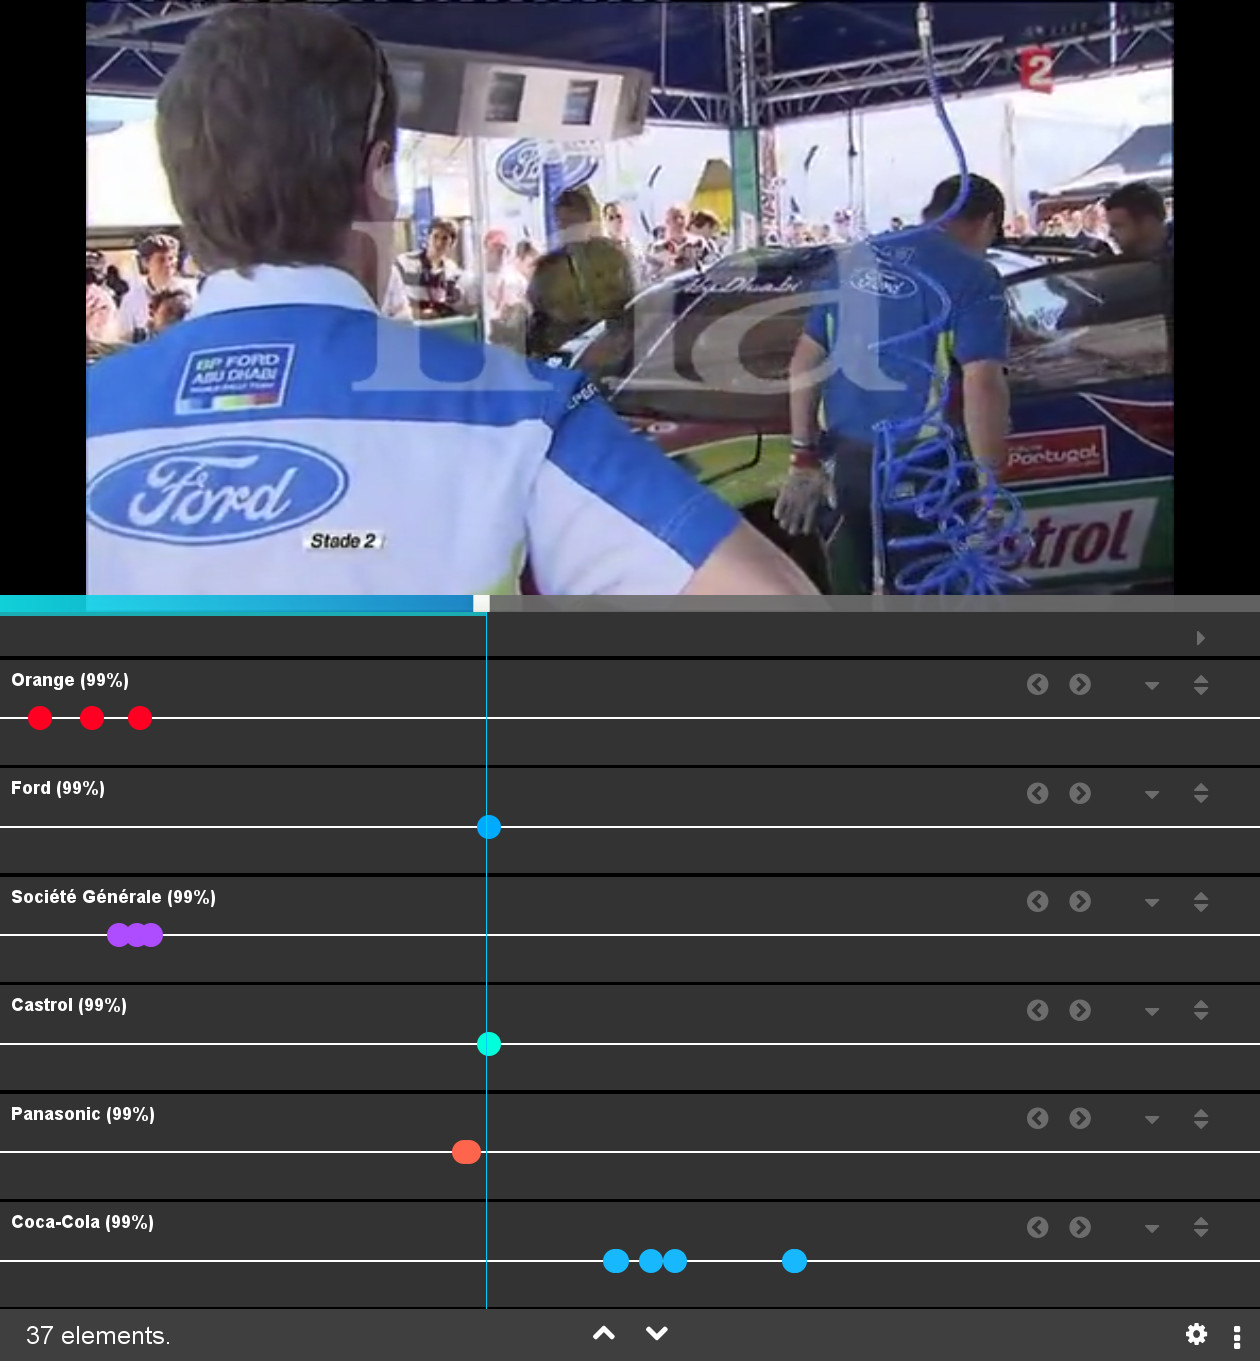
\includegraphics[width=10cm]{images/diginpix_resultat.jpg}
	\caption[Extraction des entités nommées d'un programme de France 2 avec DigInPix]{Extraction des entités nommées d'un programme de France 2 avec DigInPix [Source: \cite{institut_national_de_laudiovisuel_diginpix_nodate}]}
	\label{diginpix_result}
\end{figure}

Avec le projet du \index[ref]{led@Linked Enterprise Data (LED)!ldd@Lac de données (INA)}\index[ref]{modelisation@Modélisation!ldd@Lac de données (INA)}\ldd, la création de descriptions de contenus peut aller encore plus loin. En effet, le modèle de données unifié, comprenant l'ensemble des anciens référentiels de la \ac{ddcol}, permet de mettre en relation les données issues automatiquement d'un processus de traitement des vidéos par l'intelligence artificielle avec les concepts du \ldd. La segmentation automatique de vidéos\footnote{Le projet est SAAJ, Segmentation et Analyse Automatique des Journaux télévisés.} montre la diversité des utilisations possibles d'un référentiel quand celui-ci est uniforme et centralisé. Ce nouveau projet, au sein de celui du \ldd, débute en 2018 et conduit à la création de multiples outils, permettant tous une description automatique du contenu d'une vidéo --- les journaux télévisés et les chaînes d'information. Ainsi, la segmentation automatique par l'intelligence artificielle permet:
\begin{itemize}
	\item l'établissement d'une grille de programmation à partir des métadonnées fournies par les diffuseurs, les producteurs, \dots afin de déterminer les horaires prévus et habituels de chaque programme pour les chaînes d'information
	\item la classification automatique du programme ou des segments de programme selon une typologie précise --- plateau, présentateur, reportage, \dots
	\item la transcription des voix et de la parole, produisant ainsi un texte non formaté à partir duquel une description du contenu est effectuée avec des entités nommées qui en sont extraites et un alignement avec les entités de Wikidata
	\item l'océrisation des textes présents dans l'image, créant également un texte qui permet une description intellectuelle du contenu et un alignement des entités nommées avec Wikidata; cette océrisation concerne notamment les bandeaux des journaux télévisés dans lesquels le nom et la fonction de chaque personne sont indiqués
	\item la description automatique d'une image par un tagging d'entités nommées
	\item la reconnaissance de visages afin d'identifier le présentateur du journal télévisé, ou les protagonistes des vidéos
	\item la reconnaissance d'images et de logos, afin d'enrichir la description déjà précise de la vidéo ou du segment
\end{itemize} 

Chacun de ces outils fonctionne avec, ou en relation avec, un ou plusieurs référentiels: ils peuvent être internes, c'est à dire propres à l'\ac{ina}, ou bien externes comme Wikidata qui permet un enrichissement et une ouverture des métadonnées vers l'extérieur. Ces données générées automatiquement sont créées sous le modèle du \index[ref]{led@Linked Enterprise Data (LED)!ldd@Lac de données (INA)}\index[ref]{modelisation@Modélisation!ldd@Lac de données (INA)}\ldd et sont, par conséquent, en relation avec ses concepts. 

\subsection{\label{III-B-3-b}Faciliter et améliorer le catalogage des documents de l’\ac{ina} par l’extraction automatique de données}
\titreEntete{Faciliter et améliorer le catalogage des documents}

L'apport du projet SAAJ est une description fine et précise de l'ensemble d'une vidéo. Au-delà de la génération automatique de métadonnées dans le \index[ref]{led@Linked Enterprise Data (LED)!ldd@Lac de données (INA)}\index[ref]{modelisation@Modélisation!ldd@Lac de données (INA)}\ldd, il devient une aide pour le technicien de gestion des contenus multimédia de l'\ac{ina}. En effet, il n'a plus à créer les métadonnées associées au document, mais à superviser leur qualité et leur véracité: \og Le documentaliste « humain » est-il destiné à
passer du statut de producteur de données à celui de contrôleur de la qualité des fruits de l’automatisation ?\fg{}\footcite[p.134]{alquier_production_2017}. Cet aspect de contrôle qualité est un usage indirect des données générées automatiquement: il est positif pour la création précise, fine et complète de métadonnées sur un programme; mais il contraint à un changement de pratiques de catalogage, où l'humain n'a plus le rôle principal, qui est intellectuel, dans lequel il décrit le document et son contenu. \\

Cette amélioration et cette facilitation du travail de catalogage a lieu depuis des données nouvelles, générées par l'intelligence artificielle. Cependant, le contrôle de la qualité des métadonnées, et leur enrichissement, peuvent également passer par un traitement \textit{a posteriori}. En effet, l'apparition du Web sémantique et son adoption par un grand nombre d'institutions a poussé l'\ac{ina}, associé à d'autres institutions, à mener le projet Qualinca entre 2012 et 2015 afin \og d'améliorer la richesse, la cohérence et l’interopérabilité des métadonnées du système documentaire de l’Ina à travers la mise en œuvre d’une activité de recherche dans le domaine des techniques de liage de données\fg{}\footcite[p.129]{alquier_production_2017}. Qualinca repose sur de nombreux enjeux, comme la possibilité de partager des identifiants communs entre les différents métiers, l'amélioration des descriptions de contenus grâce aux données extérieures du \index[ref]{lod@Linked Open Data (LOD)}\ac{lod}, mais également d'effacer les ambiguïtés des termes des lexiques de l'\ac{ina}.\\

Se basant sur deux algorithmes, ProbFr et Agreg, Qualinca s'est surtout tourné vers les alignements de corpus de musique, et d'homonymes de personnes physiques et d'émissions. Dans cet alignement des homonymes avec le \index[ref]{lod@Linked Open Data (LOD)}\ac{lod}, la base \index[ref]{lod@Linked Open Data (LOD)!dbpedia@DBpédia}DBpedia --- Wikidata n'est né qu'en 2014 ---, les résultats sont peu exploitables et se heurtent, comme nous avons pu le constater lors de l'alignement des personnes physiques avec Wikidata, au langage naturel des fonctions que les algorithmes sont incapables de dépasser: sur 5000 \nP{Jacques}{Martin}, 667 différents ont été identifiés par les algorithmes\footcite[p.133]{alquier_production_2017}.\\

L'extraction automatique d'entités nommées a permis la création de nouvelles métadonnées, associées non pas au matériel ou aux données de diffusion mais au contenu intellectuel des vidéos, ainsi que l'apport d'une aide au \index[ref]{led@Linked Enterprise Data (LED)!ldd@Lac de données (INA)}\index[ref]{modelisation@Modélisation!ldd@Lac de données (INA)}catalogage par la qualité des entités fournies et leur précision.

\subsection{\label{III-B-3-c}Améliorer la valorisation des documents et offrir une meilleure expérience utilisateur}
\titreEntete{Améliorer la valorisation des documents}

La centralisation des données de l'\ac{ina} au sein du \index[ref]{led@Linked Enterprise Data (LED)!ldd@Lac de données (INA)}\index[ref]{modelisation@Modélisation!ldd@Lac de données (INA)}\ldd ouvre des possibilités pour la valorisation des documents auprès de tous les publics\footnote{Pour l'ensemble de l'offre disponible, voir la \reference{I-B}.}. D'abord, cette centralisation permet la création de multiples applications pour l'utilisateur, sans que cela ne modifie la structure des données\footnote{Voir \reference{annexe_lac} (\reference{lac_infra}).}; ainsi, la présence de l'\ac{ina} en est modifiée par l'apparition d'un \textit{hub} regroupant l'ensemble de l'offre numérique de l'Institut\footnote{\og L’autre grand défi posé à l’Institut, c’est celui de l’accessibilité de ses propositions. Les rassembler au sein d’un grand portail numérique, un hub qui offrira en quelques clics un accès renouvelé, simplifié et cohérent à l’ensemble des activités, contenus et services de l’Ina, est ainsi l’objectif qui mobilise aujourd’hui toute l’entreprise à l’horizon de 2019.\fg{} in \cite{vallet_ina_nodate}}.\\

Cette centralisation de l'offre est aussi présente pour les usages internes avec la création d'une nouvelle interface de consultation des métadonnées et des documents en eux-mêmes, Notilus, afin d'éviter la consultation croisée de multiples interfaces selon la provenance du document comme cela était le cas avant le \index[ref]{led@Linked Enterprise Data (LED)!ldd@Lac de données (INA)}\index[ref]{modelisation@Modélisation!ldd@Lac de données (INA)}\ldd. Par cette interface, le \ac{dl}, le \ac{da}, puis la \ac{dj} et l'ensemble des professionnels de l'\ac{ina}, ont accès aux mêmes données et aux mêmes documents, en un point unique, une interface de consultation qui reconstitue les instances du \ldd.\\

L'amélioration de l'expérience utilisateur est également une priorité dans une période où la modification des pratiques est radicale: ces pratiques sont quasiment toutes numériques et contraignent l'\ac{ina} à s'adapter. Si le site \url{https://www.ina.fr} est né dès 2009, le \index[ref]{led@Linked Enterprise Data (LED)!ldd@Lac de données (INA)}\index[ref]{modelisation@Modélisation!ldd@Lac de données (INA)}\ldd va pouvoir lui apporter d'importantes améliorations. En effet, la présence des référentiels y est limitée et restreint les possibilités de rebonds de la part de l'utilisateur\footnote{Voir \reference{inafr_result}.}. Ainsi, les liens des personnes au générique ne renvoient pas à une vedette personne de l'\ac{ina}, mais à des résultats de recherche sur le nom de cette personne. 
\begin{figure}[!h]
	\centering
	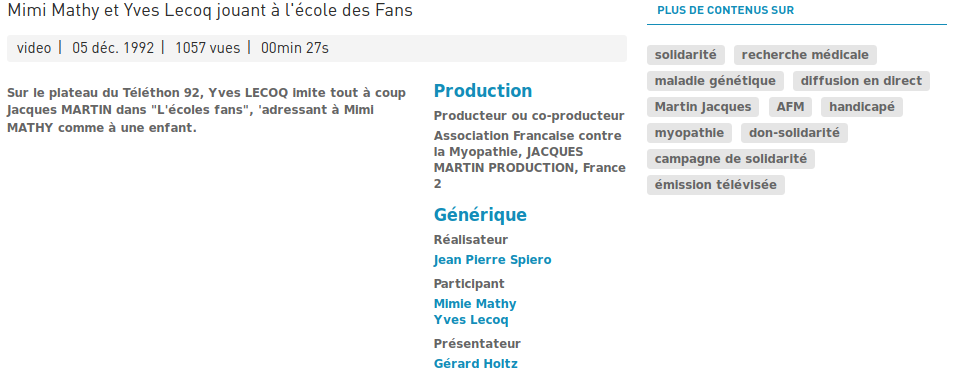
\includegraphics[width=13cm]{images/inafr_ecole_fans.png}
	\caption[Métadonnées associées à un document sur ina.fr]{Métadonnées associées à un document sur ina.fr [Source: \url{https://www.ina.fr/video/I11297765/mimi-mathy-et-yves-lecoq-jouant-a-l-ecole-des-fans-video.html}]}
	\label{inafr_result}
\end{figure}\\
Les possibilités offertes par le \ldd sont multiples et nous pouvons en imaginer certaines, basées sur le seul usage des concepts et de leurs relations, qui faciliteraient la recherche de l'utilisateur. Ainsi, comme pour la BnF, la création de vedettes de personnes est envisageable afin de regrouper en une même page les informations biographiques, ainsi que les documents liés (les instances) ou bien les thématiques principales (les concepts liés). Les termes d'indexation et de description des vidéos peuvent également être concernés par ce regroupement d'informations et de liens. Cependant, plus encore que ces regroupements de métadonnées, d'instances et de concepts relatifs à un concept, il est désormais possible, par les liens établis avec le \index[ref]{lod@Linked Open Data (LOD)}\ac{lod}, d'obtenir des informations manquantes et d'enrichir les données proposées à l'utilisateur: un lien peut être inséré, comme c'est le cas dans \index[ref]{lod@Linked Open Data (LOD)!viaf@VIAF}\index[ref]{autorites@Autorités!viaf@VIAF}\ac{viaf}, ou bien les champs peuvent être directement remplis sur la page HTML.\\

Ces possibilités ne sont envisageables que par la déconstruction de l'information dans le \ldd, permettant alors une grande modularité des données dans les usages qui en sont faits. Ces usages ne sont pas tous nés et le \index[ref]{led@Linked Enterprise Data (LED)!ldd@Lac de données (INA)}\index[ref]{modelisation@Modélisation!ldd@Lac de données (INA)}\ldd doit pouvoir permettre à l'\ac{ina} de les remplir sans avoir recours à un modification du modèle de données ou à la création d'une nouvelle de données. Ainsi, s'il est nécessaire de publier les données\footnote{Cet aspect semble difficile pour l'\ac{ina} en raison des données personnelles qui y sont conservées. Cependant, la loi de 2016 pour une République numérique (\cite{noauthor_loi_2016}) encourage à la publication des données de référence qui peuvent être réutilisées par d'autres services ou d'autres institutions.} sur le Web et plus particulièrement sur le Web de données, une représentation \index[ref]{echanges@Échanges!formats@Formats!rdf@RDF}\ac{rdf} est possible; avec la forte présence de l'\ac{ina} sur les réseaux sociaux, il peut être envisager de créer des publications automatiquement à partir de tags issus de concepts; \dots

%conclu
\bigskip
\bigskip
Le référentiel a atteint une place centrale dans le \ldd: l'ensemble des applications et des sites de l'Institut fonctionnent, ou vont fonctionner, depuis ce silo de métadonnées qui a été pensé selon la donnée et non plus selon les besoins. Ces derniers, évolutifs et dépendants de la période, ne peuvent pas tous être prédits, ce qui a conduit à la constitution d'un modèle de données souple et d'un processus intermédiaire de traitement de ces données, de manière à offrir à chaque application les données qui lui sont nécessaires.
